\documentclass[11pt,a4paper]{article}
\usepackage[utf8]{inputenc}
\usepackage[margin=2.4cm]{geometry}
\usepackage{amsmath,amssymb,amsthm,mathtools}
\usepackage{booktabs}
\usepackage[expansion=false]{microtype}
\usepackage[most]{tcolorbox}
\usepackage{tikz}
\usepackage{quantikz}
\usepackage[hidelinks]{hyperref}
\setlength{\parskip}{0.45em}
\setlength{\parindent}{0pt}

\providecommand{\ket}[1]{\lvert #1\rangle}
\providecommand{\bra}[1]{\langle #1\rvert}
\newcommand{\Tr}{\operatorname{Tr}}
\newcommand{\Q}{\mathbb{Q}}
\newcommand{\gr}[1]{\textsf{[#1]}}
\newcommand{\tc}{\textsf{[to confirm]}}

\tcbset{defbox/.style={colback=blue!3,colframe=blue!45!black,boxrule=0.5pt,arc=1pt,left=6pt,right=6pt,top=4pt,bottom=4pt,fonttitle=\bfseries\small}}
\tcbset{exbox/.style={colback=gray!4,colframe=gray!55,boxrule=0.4pt,arc=1pt,left=6pt,right=6pt,top=4pt,bottom=4pt,fonttitle=\bfseries\small}}
\tcbset{whybox/.style={colback=green!3,colframe=green!35!black,boxrule=0.4pt,arc=1pt,left=6pt,right=6pt,top=4pt,bottom=4pt,fonttitle=\bfseries\small}}
\newtcolorbox{defn}[1]{defbox,title={Definition. #1}}
\newtcolorbox{ex}[1]{exbox,title={Example. #1}}
\newtcolorbox{why}[1]{whybox,title={Why. #1}}

\title{The Logical State Space\\[0.3em]\large A first description, built on three small examples}
\author{Charbel Dargham}
\date{28 October 2026}

\begin{document}
\maketitle

\begin{abstract}
This document is an attempt at a compilation of the ideas I have had so far about a construction I call the \emph{Logical State Space}. The construction is meant to play, for algorithms, the role that a connectome plays for a brain: a structure from which behaviour can be read. Every piece of it is introduced together with three running examples, breadth-first search on small graphs, quantum teleportation and the BB84 key-distribution protocol, so that each definition is seen at work as soon as it appears. The document states definitions and choices, the reasons for them, what has been computed on the examples, and what is still open. It proves no theorem; it sets the stage for experiments and for the theory that should follow them.
\end{abstract}

\section*{How to read this document}

Each concept is introduced in the same way: a definition, the reason I chose it (in a green box), and its form on the running examples (in grey boxes). Sources carry a grade. Grade A means the source was opened and checked; grade B means it is known and was not re-checked; grade C means a standard textbook result cited without reopening the book. Passages marked \tc{} are modelling choices made while working out the examples that I have not yet fixed; they are the places where the examples could be built differently. All invariants reported for the examples were computed exactly with Macaulay2 (version 1.26, over $\Q$) or numerically with the stated precision.

\tableofcontents

\section{The question and the idea}\label{sec:idea}

A connectome is the map of the connections of a nervous system: neurons as nodes, synapses as links \gr{A: Sporns--Tononi--Kötter 2005}. Its point is that the structure of the map says something about how the brain behaves: there are theorems relating structure to function, such as the fixed-point rules for threshold-linear networks \gr{A: Curto--Geneson--Morrison 2018}, and higher-order structure has been read with simplicial complexes \gr{A: Giusti--Ghrist--Bassett 2016; Reimann et al.\ 2017}.

\begin{why}{The connectome idea}
If a connectome shows the structure of a brain and lets us deduce how this brain behaves, I want to construct a structure that lets us see how algorithms behave, and correlate structural properties of that structure with the behaviour of the algorithm. One behaviour matters most to me: whether the quantum circuit that runs an algorithm can be simulated efficiently by a classical computer (whether it can be \emph{dequantized}). Why a connectome-like structure of an algorithm should tell us that is exactly the question I am trying to answer; the construction is the tool for asking it, and the experiments are how we find out.
\end{why}

The object of the construction is the \emph{algorithm} that solves a problem, not the problem itself, because dequantization is a property of how a computation is carried out. For a problem $P$ and an algorithm solving it, I write $L(P)$ for its Logical State Space. It has two axes. The \emph{temporal axis} follows the algorithm step by step. The \emph{relational axis} is made of \emph{layers}: layer $0$ is how the inputs are related to one another before the algorithm does anything; layer $1$ is how the algorithm connects them, the first-order relations; layer $2$ and above hold relations of higher order. On every layer and at every time, three things are attached: a hypergraph (which variables are related), a sheaf $F$ (what the related variables actually are, their states or values), and a dynamics $\Phi$ (how those states change). An algebraic object, the toric ideal of the hypergraph, then turns the structure into invariants.

\section{The three running examples}\label{sec:examples}

\subsection{Breadth-first search}

\begin{defn}{Breadth-first search \gr{C}: Cormen--Leiserson--Rivest--Stein, \emph{Introduction to Algorithms}, 3rd ed., \S22.2}
Given a graph $G=(V,E)$ and a start vertex $s$, breadth-first search (BFS) computes, for every vertex $v$, its distance $d[v]$ from $s$ (the least number of edges on a path from $s$ to $v$). It keeps a first-in first-out queue $Q$. Initially $d[s]=0$, $d[v]=\infty$ for $v\neq s$, and $Q=(s)$. While $Q$ is not empty, it removes the first vertex $u$ of $Q$, and for each neighbour $w$ of $u$ in a fixed order, if $d[w]=\infty$ it sets $d[w]:=d[u]+1$ and appends $w$ to $Q$.
\end{defn}

I use two graphs: the $4$-cycle $C_4$, and the \emph{domino}, two squares sharing an edge, on six vertices. In both, $s=1$ and neighbours are visited in increasing order.

\begin{center}
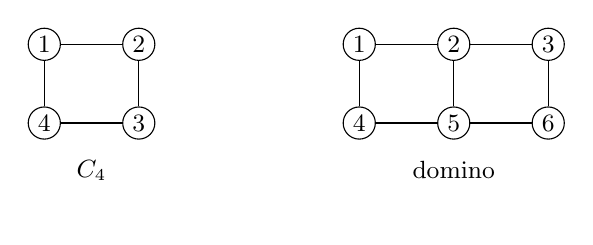
\begin{tikzpicture}[scale=1.0,every node/.style={circle,draw,inner sep=1.5pt,font=\small}]
\node (a1) at (0,1) {1}; \node (a2) at (1.2,1) {2}; \node (a3) at (1.2,0) {3}; \node (a4) at (0,0) {4};
\draw (a1)--(a2)--(a3)--(a4)--(a1);
\node[draw=none] at (0.6,-0.6) {$C_4$};
\begin{scope}[xshift=4cm]
\node (1) at (0,1) {1}; \node (2) at (1.2,1) {2}; \node (3) at (2.4,1) {3};
\node (4) at (0,0) {4}; \node (5) at (1.2,0) {5}; \node (6) at (2.4,0) {6};
\draw (1)--(2)--(3)--(6)--(5)--(4)--(1); \draw (2)--(5);
\node[draw=none] at (1.2,-0.6) {domino};
\end{scope}
\end{tikzpicture}
\end{center}

\subsection{Quantum teleportation}

A few notions are needed for the two quantum examples \gr{C: Nielsen--Chuang 2010, Ch.~1--2}. A \emph{qubit} is a unit vector $\alpha\ket0+\beta\ket1\in\mathbb{C}^2$; measuring it in the basis $\{\ket0,\ket1\}$ gives $0$ with probability $|\alpha|^2$ and $1$ with probability $|\beta|^2$, after which the qubit is in the state that was observed. Several qubits live in the tensor product of their spaces. A \emph{gate} is a unitary matrix applied to one or more qubits. The ones used here are $X=\begin{psmallmatrix}0&1\\1&0\end{psmallmatrix}$ (bit flip), $Z=\begin{psmallmatrix}1&0\\0&-1\end{psmallmatrix}$ (phase flip), the Hadamard gate $H=\tfrac1{\sqrt2}\begin{psmallmatrix}1&1\\1&-1\end{psmallmatrix}$, which sends $\ket0$ to $\ket+=(\ket0+\ket1)/\sqrt2$ and $\ket1$ to $\ket-=(\ket0-\ket1)/\sqrt2$, and the controlled-NOT gate $\mathrm{CNOT}$ on two qubits, which applies $X$ to the second (the \emph{target}) exactly when the first (the \emph{control}) is $\ket1$: $\ket{c,t}\mapsto\ket{c,t\oplus c}$. The Bell state $\ket{\beta_{00}}=(\ket{00}+\ket{11})/\sqrt2$ is the standard maximally entangled state of two qubits.

\begin{defn}{Quantum teleportation \gr{C}: Bennett et al.\ 1993; circuit of Nielsen--Chuang 2010, \S1.3.7}
Alice holds a qubit $q_0$ in an unknown state $\ket\psi=\alpha\ket0+\beta\ket1$, and she and Bob share a Bell pair: Alice holds $q_1$, Bob holds $q_2$, in the state $\ket{\beta_{00}}$. The protocol has six steps. (1) Alice applies $\mathrm{CNOT}$ with control $q_0$ and target $q_1$. (2) Alice applies $H$ to $q_0$. (3) Alice measures $q_0$ and $q_1$, obtaining bits $m_1,m_2$. (4) Alice sends $m_1,m_2$ to Bob over an ordinary classical channel; Bob's copies are $m_1',m_2'$. (5) Bob applies $X$ to $q_2$ if $m_2'=1$. (6) Bob applies $Z$ to $q_2$ if $m_1'=1$. At the end $q_2$ is in the state $\ket\psi$.
\end{defn}

\begin{center}
\begin{quantikz}[row sep=0.25cm, column sep=0.35cm]
\lstick{$q_0:\ket\psi$} & \ctrl{1} & \gate{H} & \meter{} & \setwiretype{c} \rstick{$m_1$} \\
\lstick[2]{$q_1,q_2:\ket{\beta_{00}}$} & \targ{} & & \meter{} & \setwiretype{c} \rstick{$m_2$} \\
 & & & & \gate{X^{m_2'}} & \gate{Z^{m_1'}} & \rstick{$\ket\psi$}
\end{quantikz}
\end{center}

\subsection{BB84 with an eavesdropper}

\begin{defn}{BB84 key distribution, one round, with an intercept--resend eavesdropper \gr{C}: Bennett--Brassard 1984; Nielsen--Chuang 2010, \S12.6.3}
Alice draws two random bits, a value $a$ and a basis $\alpha$, and prepares a qubit $q$ from $\ket0$ by applying $X^{a}$ and then $H^{\alpha}$: the value is encoded in the standard basis if $\alpha=0$ and in the basis $\{\ket+,\ket-\}$ if $\alpha=1$. Eve, the eavesdropper, draws a basis bit $\varepsilon$, measures $q$ in that basis (apply $H^{\varepsilon}$, measure, obtain $e$), and resends a fresh qubit prepared in the same way from $e$ and $\varepsilon$. Bob draws a basis bit $\beta$, applies $H^{\beta}$ and measures, obtaining $r$. Alice and Bob then announce their bases publicly (Bob receives a copy $\alpha'$ of $\alpha$, Alice a copy $\beta'$ of $\beta$), each computes whether the bases agree ($\kappa_B=[\alpha'=\beta]$, $\kappa_A=[\alpha=\beta']$), keeps the bit only if they do ($s_A$ from $a$, $s_B$ from $r$), and Alice announces $s_A$ (Bob's copy $s_A'$) so that Bob can compute the error bit $\mathit{err}=[s_A'\neq s_B]$.
\end{defn}

The bases are agreed upon in half the rounds; on those rounds, if Eve intercepts every round, the error rate is $1/4$, whereas it is $0$ without her \gr{C: Nielsen--Chuang 2010, \S12.6.3}. An exact enumeration over the sixteen choices of $(a,\alpha,\varepsilon,\beta)$ confirms both numbers. This error rate is how the protocol detects the eavesdropper, and it is the behaviour of BB84 that a structure should eventually account for.

\section{Algorithms, variables, operations and terms}\label{sec:terms}

\begin{defn}{Variables, domains and operations}
An algorithm acts on \emph{variables}. Each variable has a \emph{domain}, the set of values it may hold, fixed by the algorithm. An \emph{operation} reads a set $S$ of variables and writes one variable $x_i$: $x_i:=G_i(x_S)$. Variables created during the run, such as intermediate results, are \emph{temporary}: they exist from the step that creates them to the step that last uses them.
\end{defn}

\paragraph{Domains.} A variable can in principle range over $\mathbb{R}$ or another infinite set, but an algorithm that can actually be run only ever uses a finite amount of information about it at any finite stage; this is the reading of computable analysis \gr{C: Weihrauch 2000}. I do not assume that a domain is a field: it can be a ring, or only a monoid, and the algebra of $L(P)$ must reflect the algorithm's own operations on it.

\begin{defn}{Terms and term functions \gr{C}: Burris--Sankappanavar 1981}
The \emph{term} of an operation is the expression the code writes, built from variables and operation symbols. Evaluating it in the domain gives its \emph{term function}, what it computes. Two terms can have the same function: on bits, $a\oplus b$ and $(a\vee b)\wedge\neg(a\wedge b)$ compute the same table with one and three operations.
\end{defn}

\begin{why}{Terms first}
I want to show \emph{how} the code computes; we do not need a Logical State Space to study \emph{what} is computed. So each relation carries the term of its operation, and its function is derived from the term.
\end{why}

\begin{ex}{Variables of the three examples}
BFS: the distance variables $d[1],\dots,d[n]$, with domain $\{0,1,\dots,n-1,\infty\}$. With the operations $\min$ and $+1$ this domain is a piece of the tropical semiring $(\mathbb{N}\cup\{\infty\},\min,+)$ \gr{C: Maclagan--Sturmfels 2015}, which is not a field: a first case where the domain is not one. The term of an update is ``\texttt{if d[w]==INF then d[u]+1 else d[w]}''. The queue $Q$ and the current vertex $u$ fix the order of the updates; I treat them as the schedule rather than as variables \tc.

Teleportation: the qubits $q_0,q_1,q_2$ (domain $\mathbb{C}^2$ each), and the classical bits $m_1,m_2$ and Bob's copies $m_1',m_2'$ (domain $\{0,1\}$), which are temporary.

BB84: the random input bits $a,\alpha,\varepsilon,\beta$, the qubit $q$, and the classical variables $e,r,\alpha',\beta',\kappa_A,\kappa_B,s_A,s_B,s_A',\mathit{err}$.
\end{ex}

\section{The two axes}\label{sec:axes}

\paragraph{The temporal axis.} Time is the sequence of the algorithm's steps, $t=1,\dots,T$. The cuts along this axis are the steps of the algorithm itself, as it is written. A loop is not a cycle in the structure: its iterations are iterands of the same command, each happening at its own time, so a loop running from $t=x_1$ to $t=x_n$ appears as a sequence of snapshots, one per iteration. At each time $t$ the structure is a snapshot; the vertices (the variables) stay the same, and what changes is which relations are active and what the variables hold. This is the setting of graph dynamical systems with a fixed graph \gr{C: Mortveit--Reidys 2008}.

\paragraph{The relational axis.} Layer $0$ records how the inputs are related without considering the algorithm. Layer $1$ records how the algorithm connects the variables, the first-order relations. Layer $2$ and above record relations of higher order. The layers are linked to one another, and Section~\ref{sec:glue} says how.

\begin{ex}{Temporal cuts}
Teleportation has six steps, the six of its definition; the two measurements of step 3 happen at the same time. BB84 has thirteen: Alice's two gates, Eve's four actions (gate, measurement, re-preparation, gate), Bob's gate and measurement, the announcement of the bases, the two comparisons, the two key bits, the announcement of $s_A$, and the error bit. BFS on $C_4$ performs three updates of $d$ (at $u=1$: $d[2]$ then $d[4]$; at $u=2$: $d[3]$), on the domino five ($d[2],d[4]$; $d[3],d[5]$; $d[6]$); each update is one step.
\end{ex}

\section{Layer zero: how the inputs are related}\label{sec:layer0}

\begin{defn}{Layer zero}
The vertices of layer zero are the true inputs of the algorithm. Its relations are how those inputs are related in the input, before any operation: for qubits, how they are entangled or correlated in the input state; for a graph given as input, the graph itself, whose nodes play the role of the qubits and whose edges play the role of their entanglement.
\end{defn}

For quantum inputs the strength of a relation is measured with entropies \gr{C: Nielsen--Chuang 2010, \S11.3}. The von Neumann entropy of a state $\rho$ is $S(\rho)=-\Tr\rho\log_2\rho$, the number of bits of uncertainty it carries; the state of a subset $A$ of qubits is the partial trace $\rho_A$ of the full state over the other qubits. The weight of a pair is the mutual information
\[ C^{(2)}_{ij}=S(\rho_i)+S(\rho_j)-S(\rho_{ij}), \]
the number of bits qubits $i$ and $j$ share \gr{A: Valdez et al.\ 2017, who use half this value}. The weight of a triple is the irreducible three-party correlation $C^{(3)}_{ijk}=S(\tilde\rho_2)-S(\rho_{ijk})$, where $\tilde\rho_2$ is the state of largest entropy with the same two-qubit marginals as $\rho_{ijk}$: the information present only in the three together \gr{C: Linden--Popescu--Wootters 2002; B: Zhou 2008}. Higher orders follow the same pattern. Layer zero is computed per input.

\begin{ex}{Layer zero of the three examples}
Teleportation: the input is $\ket\psi\otimes\ket{\beta_{00}}$ on $q_0,q_1,q_2$. Since $q_0$ is in a pure state independent of the others, $C^{(2)}_{01}=C^{(2)}_{02}=0$, and since $q_1,q_2$ form a Bell pair, $C^{(2)}_{12}=2$ bits, the largest possible value for two qubits; the triple weight is $0$. Layer zero is one edge, $\{q_1,q_2\}$ of weight $2$, and the isolated vertex $q_0$. This is computed for every $\ket\psi$ and confirmed numerically.

BB84: the inputs $a,\alpha,\varepsilon,\beta$ are independent random bits and $q$ starts in $\ket0$; every weight is $0$, so layer zero has five vertices and no relation. The structure of BB84 is entirely created by the protocol.

BFS: layer zero is the input graph, $C_4$ or the domino, unweighted.
\end{ex}

\section{Layer one: how the algorithm connects the variables}\label{sec:layer1}

\begin{defn}{Layer one}
The vertices of layer one are the variables of the algorithm. Each operation $x_i:=G_i(x_S)$ performed at time $t$ gives a \emph{directed hyperedge} $S\to i$ active at time $t$, whose vertex set is $S\cup\{i\}$ and which carries the term of the operation. An operation that acts on several variables at once gives a single hyperedge; operations performed one after another give separate hyperedges at different times. Faces are not filled in: a hyperedge on three variables does not create the pairs it contains. A measurement is an operation from a qubit to a classical bit; sending a bit to another party is an operation from the bit to its copy.
\end{defn}

\begin{why}{Simultaneous versus sequential}
Sequential operations are handled by the dynamics, along the temporal axis. A simultaneous operation happens in one time frame, and at that time the variables it involves are connected together: that is a genuine higher-order relation, so it is one hyperedge.
\end{why}

\begin{why}{Directions}
A CNOT does not treat its two qubits alike: the control decides, the target is changed. Forgetting the direction would forget how the gate works, so hyperedges are directed, from the variables read to the variable written.
\end{why}

\begin{ex}{Layer one of teleportation, step by step}
$t=1$: $\{q_0,q_1\}\to q_1$, term $\mathrm{CNOT}$ with control $q_0$ and target $q_1$ (the new value of $q_1$ depends on both). $t=2$: $\{q_0\}\to q_0$, term $H$. $t=3$: $\{q_0\}\to m_1$ and $\{q_1\}\to m_2$, two measurements at the same time, kept as two hyperedges because they are two operations \tc. $t=4$: $\{m_1\}\to m_1'$ and $\{m_2\}\to m_2'$. $t=5$: $\{m_2',q_2\}\to q_2$, term $X^{m_2'}$. $t=6$: $\{m_1',q_2\}\to q_2$, term $Z^{m_1'}$.
\end{ex}

\begin{ex}{Layer one of BB84, step by step}
$\{a,q\}\to q$ ($X^a$); $\{\alpha,q\}\to q$ ($H^\alpha$); $\{\varepsilon,q\}\to q$; $\{q\}\to e$; $\{e\}\to q$ (re-preparation after reset) \tc; $\{\varepsilon,q\}\to q$; $\{\beta,q\}\to q$; $\{q\}\to r$; $\{\alpha\}\to\alpha'$ and $\{\beta\}\to\beta'$; $\{\alpha',\beta\}\to\kappa_B$ and $\{\alpha,\beta'\}\to\kappa_A$; $\{\kappa_A,a\}\to s_A$ and $\{\kappa_B,r\}\to s_B$; $\{s_A\}\to s_A'$; $\{s_A',s_B\}\to\mathit{err}$. The comparisons read two variables at once and give hyperedges of size three.
\end{ex}

\begin{ex}{Layer one of BFS}
Each update $d[w]:=d[u]+1$ gives the hyperedge $\{d[u],d[w]\}\to d[w]$. A test that finds $d[w]\neq\infty$ writes nothing and gives no hyperedge \tc. On $C_4$ the hyperedges are $\{d_1,d_2\},\{d_1,d_4\},\{d_2,d_3\}$; on the domino $\{d_1,d_2\},\{d_1,d_4\},\{d_2,d_3\},\{d_2,d_5\},\{d_3,d_6\}$. Over the whole run they form the BFS tree, while layer zero holds the whole input graph: the algorithm uses only part of the input's relations.
\end{ex}

\section{Higher layers}\label{sec:higher}

Layer $k\ge2$ holds relations of order $k$: relations among the relations of the layer below. On the three examples, the relations among layer-one hyperedges that the algebra of Section~\ref{sec:algebra} detects are exactly where such relations could come from; the rule that produces layer $2$ from layer $1$ is not yet defined, and it is the first open problem of Section~\ref{sec:open}.

\section{The sheaf $F$: what the related variables are}\label{sec:sheaf}

\begin{defn}{The sheaf $F$}
To every set $\sigma$ of variables, $F$ assigns the possible joint states of those variables, and to every inclusion $\tau\subseteq\sigma$ a restriction map $F(\sigma)\to F(\tau)$ that forgets the variables not in $\tau$. For qubits, $F(\sigma)$ is the set of density operators on $\bigotimes_{q\in\sigma}\mathbb{C}^2$ and the restriction is the partial trace \gr{C: Nielsen--Chuang 2010, \S2.4}. For classical variables, $F(\sigma)$ is the set of probability distributions on their joint values and the restriction is marginalisation \gr{B: Abramsky--Brandenburger 2011}. For a mix of the two, $F(\sigma)$ is the set of classical--quantum states, block-diagonal operators with one quantum block per classical value \gr{C: Wilde 2017}. On the hypergraph, $F$ is read on vertices and hyperedges \tc.
\end{defn}

\begin{why}{A sheaf at all}
I need a way to go from graph theory to the actual mechanics and description of the nodes. Without $F$ the nodes and edges have no content: if I cannot take three nodes that are qubits and output their density matrix, there is no reason to construct the structure at all. The hypergraph and the physics would be two islands without a bridge; $F$ is the bridge.
\end{why}

\begin{ex}{$F$ on the examples}
Teleportation at $t=0$: $F(\{q_1,q_2\})=\ket{\beta_{00}}\bra{\beta_{00}}$, whose restrictions $F(\{q_1\})=F(\{q_2\})=I/2$ are maximally mixed: each half of a Bell pair alone looks completely random. BB84 after Bob's measurement: $F(\{a,r\})$ is a distribution on two bits, which on rounds with agreeing bases has $a\neq r$ with probability $1/4$ when Eve intercepts. BFS: the input is fixed, so every $F(\sigma)$ is a single point, the current values of the distances.
\end{ex}

\section{The dynamics $\Phi$}\label{sec:phi}

\begin{defn}{The dynamics $\Phi$}
$\Phi$ is a local rule in discrete time: at step $t$, each active hyperedge $S\to i$ replaces the state of its variables by the result of its operation, and nothing else changes. The schedule, which operations happen at which time, is given by the algorithm and is not a modelling choice. On quantum variables an operation acts on $F$ by $\rho\mapsto U\rho U^\dagger$ for a gate $U$, and a measurement acts as the channel that keeps the diagonal in the measured basis and records the outcome in a classical variable \gr{C: Nielsen--Chuang 2010, \S2.2 and \S8.2}. On classical variables it applies the term function.
\end{defn}

\begin{why}{Discrete time}
That is how algorithms work: they proceed by steps. Continuous time makes no sense for them.
\end{why}

\begin{ex}{$\Phi$ moving correlations in teleportation}
Following $F$ through the steps shows the correlations being moved. Write $H_2(p)=-p\log_2p-(1-p)\log_2(1-p)$. Before the protocol, $C^{(2)}_{12}=2$ and the other pairs are $0$. After the CNOT the computed values are $C^{(2)}_{01}=C^{(2)}_{02}=H_2(|\alpha|^2)$ and $C^{(2)}_{12}=2-H_2(|\alpha|^2)$; the Hadamard on $q_0$ acts on one qubit only and changes none of them. These values were computed for two random states $\ket\psi$ and agree with the formulas to four decimals; deriving the formulas by hand is a good exercise. After the measurements, the bits $(m_1,m_2)$ share exactly one bit with $q_2$: given the bits, $q_2$ is in the pure state $X^{m_2}Z^{m_1}\ket\psi$, and without them it is maximally mixed. The corrections then remove that dependence and leave $q_2$ in $\ket\psi$.
\end{ex}

\begin{ex}{$\Phi$ in BFS}
The distances evolve by the term function $d[w]\mapsto d[u]+1$ applied when $d[w]=\infty$, in the order the queue gives. On $C_4$ the final values are $d=(0,1,2,1)$; on the domino $d=(0,1,2,1,2,3)$.
\end{ex}

\section{The algebra: toric ideals}\label{sec:algebra}

\begin{defn}{Toric ideal of a hypergraph \gr{C}: Sturmfels 1996, Ch.~4; \gr{A}: Petrović--Stasi, \emph{Toric algebra of hypergraphs}}
Let $H$ be a hypergraph on vertices $1,\dots,n$ with hyperedges $e_1,\dots,e_r$ (direction forgotten), and let $x^{e}=\prod_{v\in e}x_v$ in $R=\Q[x_1,\dots,x_n]$. Let $S=\Q[t_{e_1},\dots,t_{e_r}]$, one variable per hyperedge, graded by $\deg t_e=|e|$. The toric ideal $I_H$ is the kernel of the ring map $S\to R$, $t_e\mapsto x^e$. It is spanned by the binomials $t^u-t^v$ for which the two monomials involve every vertex the same number of times.
\end{defn}

A generator of $I_H$ is a balanced collection of interactions: colour the hyperedges of one side red and of the other blue; every vertex meets as many red as blue \gr{A: Petrović--Stasi, Thm~2.8}. These are relations among interactions. Their own relations are the \emph{syzygies}, recorded by the minimal graded free resolution of $S/I_H$ and its graded Betti numbers $\beta_{i,j}$, the number of relations of homological order $i$ in degree $j$ \gr{C: Eisenbud 1995; Peeva 2011}. Nested hyperedges keep their own variables, so a relation on three variables survives next to relations on two of them; this is why the toric ideal is used rather than the edge ideal, which erases the larger of two nested relations. The toric ideal is used on every layer.

\begin{why}{Algebra and topology together}
I want both the relations of relations and the topology, and the toric ideal gives both. Its syzygies are the relations of relations; and its multigraded Betti numbers are ranks of reduced homology groups of simplicial complexes attached to each multidegree, a result of Campillo--Marijuán, Campillo--Pisón and Aramova--Herzog \gr{A: as stated in Favacchio--Hofscheier--Keiper--Van Tuyl}. So the algebra carries its own topology, and no second, unrelated object is needed.
\end{why}

\begin{ex}{Toric ideals of the examples (computed exactly)}
Layer zero of BFS. For $C_4$, $I=(t_{12}t_{34}-t_{23}t_{14})$: the two pairs of opposite edges balance each other; Betti numbers $\beta_{0,0}=1$, $\beta_{1,4}=1$. For the domino, $I=(t_{12}t_{45}-t_{14}t_{25},\ t_{23}t_{56}-t_{25}t_{36})$, one relation per square; the outer six-cycle gives no new relation, and the two generators have one syzygy: $\beta_{0,0}=1$, $\beta_{1,4}=2$, $\beta_{2,8}=1$.

Layer one of BFS. The BFS trees of $C_4$ and of the domino have toric ideal $0$: a tree has no balanced collection of edges. The input has relations among its relations; the algorithm's own first-order structure has none.

Teleportation and BB84. Each snapshot contains one or two hyperedges and has toric ideal $0$. The unions of consecutive snapshots used by the temporal axis (Section~\ref{sec:time}) also have toric ideal $0$, with one exception in BB84: the union of Eve's measurement $\{q\}\to e$ and her re-preparation $\{e\}\to q$ has the relation $t_{qe}^{(\mathrm{meas})}-t_{qe}^{(\mathrm{prep})}$, because the two hyperedges have the same vertex set and opposite directions, which the toric ideal cannot tell apart.
\end{ex}

\section{Weights and persistence}\label{sec:pers}

Layer zero of quantum inputs is weighted, and a toric ideal needs each hyperedge to be present or absent. The way through is a \emph{filtration}: lower a threshold step by step and let the hyperedges whose weight exceeds it enter, strongest first \gr{C: Edelsbrunner--Letscher--Zomorodian 2002}. Three filtrations are used: by the actual values, by rank, and on a fixed grid. Along a filtration $H_1\subseteq\cdots\subseteq H_m$ the toric ideals are included in one another, $I_{H_s}=I_{H_m}\cap\Q[t_e:e\in H_s]$ \gr{C: Sturmfels 1996, Ch.~4}, and the \emph{persistent Betti number} $\beta^{s,t}_{i,j}$ is the rank of the induced map from the Betti groups at stage $s$ to those at stage $t$, the same pattern as for persistent edge ideals \gr{A: Suwayyid--Wei, abstract}. Layer-one hyperedges carry no weight, so on layer one persistence lives only along the temporal axis.

\begin{ex}{Persistence on the examples}
Teleportation's layer zero has one weight, $2$ on $\{q_1,q_2\}$: the filtration has one step and the toric ideal stays $0$. BB84's layer zero is empty. BFS's layer zero is unweighted. The examples of this document are therefore too small for persistence to show anything; the learning problems of Section~\ref{sec:learning} are where it is used.
\end{ex}

\section{The temporal axis: zigzag persistence}\label{sec:time}

The snapshots along time are linked through their unions, $H_1\to H_1\cup H_2\leftarrow H_2\to H_2\cup H_3\leftarrow\cdots$, a zigzag; applying an invariant to every term and every map gives a zigzag module, whose barcode records which features are born and which die as time passes \gr{C: Carlsson--de Silva 2010}.

\begin{why}{Zigzag rather than one big network}
Building the whole history into one large static network (the time-stamped layers of Kivelä et al.\ \gr{A}) answers ``what is the whole history as one structure''. Zigzag persistence answers ``which structure persists through the history'', and it allows things to disappear, which temporary variables do. That second question is the one I want.
\end{why}

\paragraph{An observation on the examples, not part of the definition.} If the snapshots of a whole run were merged into one hypergraph, new relations would appear. For teleportation the merged hypergraph has the single relation $t_{q_0}^2\,t_{q_1m_2}\,t_{m_1m_1'}\,t_{m_2'q_2}-t_{q_0q_1}\,t_{q_0m_1}\,t_{m_2m_2'}\,t_{m_1'q_2}$, which links Alice's gates, both measurements, the channel and both corrections. For BB84 the merged hypergraph has exactly two relations, $t^{(\mathrm{meas})}_{qe}-t^{(\mathrm{prep})}_{qe}$ and $t^{(\text{first})}_{\varepsilon q}-t^{(\text{second})}_{\varepsilon q}$, and both involve only Eve's operations. Whether merging belongs in the construction is not decided.

\section{Gluing the layers}\label{sec:glue}

Layers share variables: layer zero's inputs are among layer one's variables, and higher layers sit on lower ones. The global object is a quotient ring built from the layers' ideals: for two layers with ideals $J$ and $K$ in a common polynomial ring $S$, it is $S/(J\cap K)$, chosen because it projects onto each layer, $S/(J\cap K)\to S/J$ and $\to S/K$ \gr{A: Francisco--Hà--Van Tuyl, exact sequence $0\to S/(J\cap K)\to S/J\oplus S/K\to S/(J+K)\to0$}.

With toric ideals the literature glues differently, and the construction has to be rebuilt in that setting. Each layer's ideal sits inside the composite exactly, $I_{H_k}=I_H\cap\Q[t_e:e\in H_k]$, and every hyperedge belongs to the one layer whose relation it records, so only vertices are shared. What the composite has beyond the layers, its \emph{twists}, is measured by the following known cases. With no twist the ideal splits, $I_H=I_{H_k}+I_{H_{k+1}}$, and its Betti numbers follow from the layers' \gr{A: Favacchio--Hofscheier--Keiper--Van Tuyl, Thm~3.5}. With exactly one twist, $I_H=I_{H_k}+I_{H_{k+1}}+\langle\rho\rangle$ (a gluing in the sense of Rosales \gr{A: as stated in García-García--Moreno-Frías--Vigneron-Tenorio}), and the resolution of the composite is the tensor product of the layers' resolutions followed by a mapping cone of multiplication by $\rho$, with the explicit formula
\[\beta_i(\text{composite})=\sum_{i'=0}^{i}\beta_{i'}(\text{layer }k)\big[\beta_{i-i'}(\text{layer }k{+}1)+\beta_{i-i'-1}(\text{layer }k{+}1)\big]\]
\gr{A: Gimenez--Srinivasan, Thm~3.1 and Cor.~3.2}. With several describable twists the toric fiber product applies \gr{A: Sullivant, abstract}; in general gluing gives a saturation \gr{A: Favacchio et al., Thm~4.5, for graphs}. On the input variables, layer zero and layer one are identified; how these two layers are glued is open.

\section{Learning problems}\label{sec:learning}

\begin{defn}{Supervised binary classification \gr{C}: Shalev-Shwartz--Ben-David 2014, Ch.~2}
A domain $\mathcal{X}$ of inputs, labels $\{-1,+1\}$, an unknown labelling function $f:\mathcal{X}\to\{-1,+1\}$, and a distribution of inputs. A learner receives labelled training examples and returns a classifier; a separate test sample estimates how often it is wrong.
\end{defn}

The Logical State Space is to be tested on learning problems from three families with different kinds of structure: properties of graphs, covariance matrices of measured signals, and phases of spin chains. The first experiment uses spin chains. Each input is the ground state of a chain of qubits (the eigenvector of lowest energy of the chain's Hamiltonian, a $2^n\times2^n$ real symmetric matrix depending on a field parameter $h$), and the label says on which side of the critical value $h=1$ the input was prepared \gr{C: Pfeuty 1970}. This task is known as quantum phase classification \gr{B: Carrasquilla--Melko 2017; Cong--Choi--Lukin 2019; Huang et al.\ 2022}.

\paragraph{Experiment A.} The question is whether the invariants of layer zero track the properties of the states that matter for their circuits (half-chain entanglement entropy, energy gap, phase) better than null models do. Layer zero is built per input on the qubits, weighted by $C^{(2)}$ and $C^{(3)}$, filtered in the three ways of Section~\ref{sec:pers}, and read through the persistent Betti numbers of the toric ideals. The data are the transverse-field Ising and XXZ chains of my spin-chain dataset, with their fixed training and test split. Still to be fixed before it runs: whether pairs and triples form one object or two, which null model, which invariant is the main one (fixed in advance), which statistical test, and which gap is tracked. A workbook computes the full layer zero of one of these problems by hand, the four-qubit transverse-field Ising ring.

\section{Next steps}\label{sec:next}

The first step is to run experiment A once its open choices are fixed. The second is the rule producing layer $2$, without which the relational axis stops at first-order relations. The third is the passage from $L(P)$ to circuits, with the comparison between the Logical State Space of a quantum algorithm and that of a classical one solving the same problem, $L_q(P)$ and $L_c(P)$, and the possibility that survival under dequantization shows up as a kind of duality between them, once the two structures can be linked computationally. Three known routes from an algorithm to a circuit will be looked at: making the computation reversible, which turns each operation $x_i:=G_i(x_S)$ into a gate on the variables $S\cup\{i\}$ \gr{C: Bennett 1973; Toffoli 1980}; the Feynman--Kitaev construction, which turns a circuit into a sum of local terms, one per gate \gr{C: Feynman 1985; Kitaev--Shen--Vyalyi 2002}; and the theorem that a circuit can be simulated classically at a cost exponential only in the treewidth of its graph \gr{B: Markov--Shi 2008}, the first known link between a structural invariant and classical simulability.

\section{Open problems}\label{sec:open}

The rule that produces layer $k+1$ from layer $k$ is not defined. Directions are carried by the hyperedges, $F$ and $\Phi$, but the toric ideal forgets them, and on BB84 this already produces a relation between two different operations of Eve's that share a vertex set; where direction enters the algebra is open. The toric gluing gives inclusions of each layer into the composite but no projections back onto the layers, which the ring $S/(J\cap K)$ was chosen to provide; whether projections survive is open. Persistent Betti numbers of toric ideals are a definition without theorems: no stability result and no formula of Hochster type along a filtration is known. The algebraic counterpart of zigzag persistence for toric ideals is not defined, and neither is whether a whole run should be merged. The algebra must reflect operations on domains that are not fields, such as the tropical domain of BFS, and this has not been worked out. The gluing of layer zero to layer one, which share the input variables, is not settled. Finally, the comparison of $L_q(P)$ and $L_c(P)$ is not defined.

\section*{References}
\small
\begin{tabular}{@{}p{0.97\textwidth}@{}}
S.~Abramsky, A.~Brandenburger, The sheaf-theoretic structure of non-locality and contextuality, \emph{New J.\ Phys.} 13 (2011). \gr{B}\\
C.~H.~Bennett, Logical reversibility of computation, \emph{IBM J.\ Res.\ Dev.} 17 (1973). \gr{C}\\
C.~H.~Bennett, G.~Brassard, Quantum cryptography: public key distribution and coin tossing, Proc.\ IEEE Int.\ Conf.\ Computers, Systems and Signal Processing (1984). \gr{C}\\
C.~H.~Bennett et al., Teleporting an unknown quantum state via dual classical and Einstein--Podolsky--Rosen channels, \emph{Phys.\ Rev.\ Lett.} 70 (1993). \gr{C}\\
S.~Burris, H.~P.~Sankappanavar, \emph{A Course in Universal Algebra}, Springer, 1981. \gr{C}\\
G.~Carlsson, V.~de~Silva, Zigzag persistence, \emph{Found.\ Comput.\ Math.} 10 (2010). \gr{C}\\
J.~Carrasquilla, R.~Melko, Machine learning phases of matter, \emph{Nature Physics} 13 (2017). \gr{B}\\
I.~Cong, S.~Choi, M.~Lukin, Quantum convolutional neural networks, \emph{Nature Physics} 15 (2019). \gr{B}\\
T.~Cormen, C.~Leiserson, R.~Rivest, C.~Stein, \emph{Introduction to Algorithms}, 3rd ed., MIT Press, 2009. \gr{C}\\
C.~Curto, J.~Geneson, K.~Morrison, Fixed points of competitive threshold-linear networks, arXiv:1804.00794. \gr{A}\\
H.~Edelsbrunner, D.~Letscher, A.~Zomorodian, Topological persistence and simplification, \emph{Discrete Comput.\ Geom.} 28 (2002). \gr{C}\\
D.~Eisenbud, \emph{Commutative Algebra with a View Toward Algebraic Geometry}, Springer, 1995. \gr{C}\\
G.~Favacchio, J.~Hofscheier, G.~Keiper, A.~Van Tuyl, Splittings of toric ideals, arXiv:1909.12820. \gr{A}\\
R.~P.~Feynman, Quantum mechanical computers, \emph{Optics News} 11 (1985). \gr{C}\\
C.~Francisco, H.~T.~Hà, A.~Van Tuyl, Splittings of monomial ideals, arXiv:0807.2185. \gr{A}\\
J.~I.~García-García, M.~A.~Moreno-Frías, A.~Vigneron-Tenorio, Combinatorial properties and characterization of glued semigroups, arXiv:1104.2835. \gr{A}\\
P.~Gimenez, H.~Srinivasan, The structure of the minimal free resolution of semigroup rings obtained by gluing, arXiv:1710.07237. \gr{A}\\
C.~Giusti, R.~Ghrist, D.~Bassett, Two's company, three (or more) is a simplex, arXiv:1601.01704. \gr{A}\\
H.-Y.~Huang et al., Provably efficient machine learning for quantum many-body problems, \emph{Science} 377 (2022). \gr{B}\\
A.~Kitaev, A.~Shen, M.~Vyalyi, \emph{Classical and Quantum Computation}, AMS, 2002. \gr{C}\\
M.~Kivelä et al., Multilayer networks, \emph{J.\ Complex Networks} 2 (2014). \gr{A}\\
N.~Linden, S.~Popescu, W.~Wootters, Almost every pure state of three qubits is completely determined by its two-particle reduced density matrices, \emph{Phys.\ Rev.\ Lett.} 89 (2002). \gr{C}\\
D.~Maclagan, B.~Sturmfels, \emph{Introduction to Tropical Geometry}, AMS, 2015. \gr{C}\\
I.~Markov, Y.~Shi, Simulating quantum computation by contracting tensor networks, \emph{SIAM J.\ Comput.} 38 (2008). \gr{B}\\
H.~Mortveit, C.~Reidys, \emph{An Introduction to Sequential Dynamical Systems}, Springer, 2008. \gr{C}\\
M.~A.~Nielsen, I.~L.~Chuang, \emph{Quantum Computation and Quantum Information}, 10th anniversary ed., Cambridge, 2010. \gr{C}\\
I.~Peeva, \emph{Graded Syzygies}, Springer, 2011. \gr{C}\\
S.~Petrović, D.~Stasi, Toric algebra of hypergraphs, arXiv:1206.1904. \gr{A}\\
P.~Pfeuty, The one-dimensional Ising model with a transverse field, \emph{Ann.\ Phys.} 57 (1970). \gr{C}\\
M.~Reimann et al., Cliques of neurons bound into cavities provide a missing link between structure and function, \emph{Front.\ Comput.\ Neurosci.} 11 (2017). \gr{A}\\
S.~Shalev-Shwartz, S.~Ben-David, \emph{Understanding Machine Learning}, Cambridge, 2014. \gr{C}\\
O.~Sporns, G.~Tononi, R.~Kötter, The human connectome: a structural description of the human brain, \emph{PLoS Comput.\ Biol.} 1 (2005). \gr{A}\\
B.~Sturmfels, \emph{Gröbner Bases and Convex Polytopes}, AMS, 1996. \gr{C}\\
S.~Sullivant, Toric fiber products, arXiv:math/0602052. \gr{A, abstract}\\
F.~Suwayyid, G.-W.~Wei, persistent edge ideals, arXiv:2512.17619. \gr{A, abstract}\\
T.~Toffoli, Reversible computing, ICALP 1980. \gr{C}\\
M.~A.~Valdez et al., Quantifying complexity in quantum phase transitions via mutual information complex networks, \emph{Phys.\ Rev.\ Lett.} 119 (2017). \gr{A}\\
K.~Weihrauch, \emph{Computable Analysis}, Springer, 2000. \gr{C}\\
M.~Wilde, \emph{Quantum Information Theory}, 2nd ed., Cambridge, 2017. \gr{C}\\
D.~L.~Zhou, Irreducible multiparty correlations in quantum states without maximal rank, \emph{Phys.\ Rev.\ Lett.} 101 (2008). \gr{B}\\
\end{tabular}
\end{document}
